\chapter{Water Distribution Networks and Reinforcement Learning}\label{chap:RLOnWDN}

In this chapter it is shown how reinforcement learning methods from \cref{chap:RL} are used as control methods on the water distribution network presented in \cref{chap:WDN}. A cost function is formulated based on minimisation of energy consumption of pumps, combined with a barrier function. System states and action is selected based on the cost function.

\cref{chap:RL} describes two learning algorithms; the on-policy learning method Sarsa and the off-policy learning method Q-learning. The Sarsa algorithm \cref{eq:sarsa} will in time learn the optimal $ \epsilon $-greedy policy, that is the Q-values will converge to some sub-optimal Q-value function. Using Q-learning will result in the convergence to an optimal policy \cite{Sutton2020}, therefore the Q-learning algorithm will be used for the remainder of the project.  

Notice from here onward, we distinguish between the height state and actual water level height, by denoting them $h(k)$ and $h_{ewh}(k)$ respectively.

\newpage \clearpage

\section{Cost Function and State-Action Selection}\label{sec:CostFuncAndState-ActionSelection}
\cref{chap:RL} presented Reinforcement Learning and the idea of maximisation a reward function to get the greatest return. The remainder of this project will discuss minimization of a cost functions rather than maximisation of a reward functions. This means that the action value becomes related to an expected cost for which lower values are better. The $\epsilon$-greedy policy should then be altered such that the next action is found based on lowest action value rather than the biggest action value:

\begin{equation}\label{eq:EpsilonGreedyMin}
	a(k) = 
	\begin{cases} 
		\underset{a'\in A}{\arg\min} \; Q\bigg(s(k),a'\bigg) & \text{exploitation with probability} \; 1-\epsilon  \\
		\text{Random action from $ \mathcal{A} $} & \text{exploration with probability} \; \epsilon 
	\end{cases},\quad \epsilon \in [0,1]
\end{equation}

The cost function $ J $ forms the basis of the optimality problem. We formulate the cost function such that the power consumed by the pumping station is minimised and on the fact that we wish to stay within some water level limits in the elevated water reservoir:

\begin{equation}\label{eq:WDN_Cost1}
	J(k+1) = P(k) + B\bigg(h_{ewr}(k+1)\bigg)  
\end{equation}  

where,
\begin{center}
	\begin{tabular}{l p{10cm} l}
		$ P(k) $ & is the power consumed by the pumping station & [\si{W}]\\
		$ B\bigg(h_{ewr}(k+1)\bigg) $ & is a barrier function & ($\cdot$)
	\end{tabular}
\end{center}

Note that the cost is based on pump power at time $ k $ and the barrier cost is evaluated at time $ k+1 $ resulting in high cost given to actions that takes the water level into the barrier. Combining \cref{eq:WDN_Cost1} and \cref{eq:WDN_Power} yields:

\begin{equation}\label{eq:CostFunctionFinal}
	J(k+1)= q(k)\bigg(\rho g h_{ewr}(k+1)+\Delta z+\lambda\bigg(q(k)\bigg)+\lambda \bigg(q(k),d(k) \bigg)\bigg) + B\bigg(h_{ewr}(k+1)\bigg) 
\end{equation}

The barrier function is  designed such that high costs is given to water levels that are outside certain heights bounds. The barrier helps in avoiding dry-out, this is important since it counteracts the minimisation of energy inclination to empty the reservoir. Avoiding dry-out also guarantees that demand will be satisfied, because demand will drain the reservoir if pumps supply insufficient water. 

%As such the barrier function counteracts the cost of using pump power, this cost-balance determined by how the barrier is designed is one of the primary tools to shape the stationary behaviour of the system.

\cref{eq:QuadBarrier} presents the quadratic polynomial barrier function used: 

%A barrier function is included in the cost function adding a high cost to the extreme upper and lower areas of the operating range of the reservoirs water level. This is a first step toward safe learning, partly safeguarding against overflow and dryout, 

\begin{equation}\label{eq:QuadBarrier}
	B\bigg(h_{ewr}(k),a,b\bigg)=\begin{cases}
		(h_{ewr}(k)-a)^{2} & \text{if} \; h_{ewr}(k) < a \\
		0 & \text{if} \; h_{ewr}(k)\in\big[a,b\big] \\
		(h_{ewr}(k)-b)^2 & \text{if} \; h_{ewr}(k) > b 
	\end{cases}
\end{equation}

With $ a $ and $ b $ being the zeros of the left and right side polynomial respectively. A example of a barrier function of this form is shown in  \cref{fig:QuadBarrierFunc1}:

\begin{figure}[h!]
	\centering
	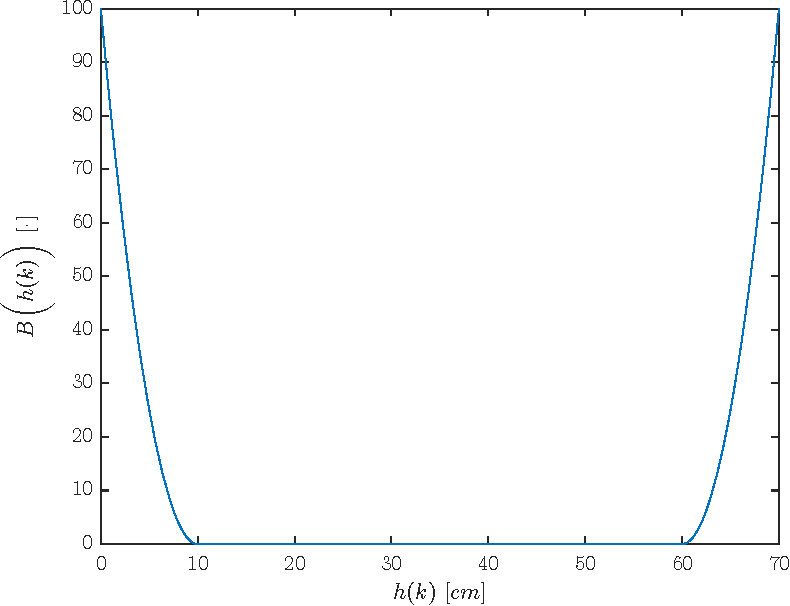
\includegraphics[width=0.7\linewidth]{Figures/QuadBarrierFuncA10B60}
	\caption{Piecewise defined quadratic barrier function from \cref{eq:QuadBarrier} with zeros in 10 and 60.}
	\label{fig:QuadBarrierFunc1}
\end{figure} 

States and action for the water distribution network reinforcement learning problem is chosen based on the cost function in \cref{eq:CostFunctionFinal}. We choose:

\begin{itemize}
	\item $ s_{1}  = h_{ewr}$: Water level of tank scales linearly to the pressure in the tank, and determines barrier cost.
	
	\item $ s_{2} = t $: Time of day. It is assumed that the consumer demand $d(k)$ behaves periodically from day to day.
	
	\item $ a = q(k) $: actions are three unique pumping-station presets, each with a different resulting flow. 
\end{itemize}


\newpage \clearpage

\section{Tabular Q-learning}\label{sec:WDNTabularQ-Learning}

For tabular Q-Learning the action values are stored in a table format: $ Q\bigg(h(k),t(k),a(k)\bigg) $. One table dimension holds discrete height states, one discrete time states and one discrete actions. 

\begin{wrapfigure}{r}{7.5cm}
	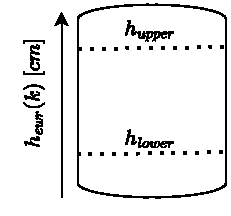
\includegraphics[width=7.5cm]{figures/HeightStates - Copy.drawio.pdf}
	\caption{Height state in elevated water reservoir.}
	\label{fig:hState}
\end{wrapfigure} 

This section explains how the states are discritised in order to fit the water distribution network described in \cref{chap:WDN}. 

Time is discretised to 24 states, matching hours of the day. A finer discretisation is not used for dimensionality issues, and it is assumed dynamics are slow enough to be captured on a hourly basis.

Discretisation of water levels in the elevated water reservoir is visualised in \cref{fig:hState}. The first and last height states consists of wider height segments than the middle states. This minimises the chance of dry-out and overflow. The water level is measured in centimetres and the height state $ h(k) $ will be chosen based on the actual water level: 

%\begin{equation} \label{eq:HeightStates}
%	h(k)=\begin{cases}
%		h_{1} & if \; h_{ewr}(k) \leq h_{Lower} \\
%		ceil\bigg(h_{ewr}(k)\bigg) & if \; h_{lower} < h_{ewr}(k) <h_{upper} \\
%		h_{n} & if \; h_{ewr}(k) \geq h_{upper} 
%	\end{cases}
%\end{equation}

\begin{equation} \label{eq:HeightStates}
	h(k)=\begin{cases}
		1 & if \; h_{ewr}(k) \leq h_{Lower} \\
		ceil\bigg(h_{ewr}(k)\bigg) & if \; h_{lower} < h_{ewr}(k) <h_{upper} \\
		h_{max} & if \; h_{ewr}(k) \geq h_{upper} 
	\end{cases}
\end{equation}

%Where $ h_{lower} $ and $ h_{upper} $ decide the region size of $ h_1 $ and $ h_n $ relative to the tank size and thereby the number of height states. $ ceil $ denotes the \textit{ceiling} function. 

Where the placements of $ h_{lower} $ and $ h_{upper} $ decide the number of height states, and the resulting upper limit of height states is denoted $ h_{max} $. $ ceil $ denotes the \textit{ceiling} function, which rounds any number to the nearest larger integer. Our use of the ceil function requires the argument to be measured in centimetres for proper height state assignment, therefore any measurement not in centimetres must first be scaled.

The number of actions is dictated by the number of pumps in the pumping station, and is by nature already discrete.

The Q-learning update law for the action value function described in \cref{eq:Q-learning} will in the case of minimising the cost function in \cref{eq:WDN_Cost1} be:

\begin{equation}\label{eq:Q-learningMin}
	\begin{split}
		Q\bigg(h(k),t(k),a(k)\bigg)\leftarrow Q\bigg(h(k),t(k),a(k)\bigg)&+\alpha \bigg[J(k+1)	+\gamma \min_{a'} Q\bigg(h(k+1),t(k+1),a'\bigg)\\
		&-Q\bigg(h(k),t(k),a(k)\bigg)\bigg]
	\end{split}
\end{equation}

with $ h(k) \in \mathcal{H} $, $ t(k) \in \mathcal{T}$ and $ a(k) \in \mathcal{A} $. That is the available states and actions belongs to closed sets. 

\cref{alg:Q-learning} presents the tabular Q-learning algorithm applied to the water distribution network presented in \cref{sec:WDNsetup}.

\begin{algorithm}
	\caption{Tabular Q-Learning algorithm}
	\label{alg:Q-learning}
	\begin{algorithmic}[1]
		\State \textbf{Input:} $\alpha\in[0,\;1]$, small $\epsilon>0$, and $0\leq\gamma < 1$ 
		\State \textbf{Initialise:} $ Q(h,t,a) $ for all $ h(k) \in \mathcal{H} $, $ t(k) \in \mathcal{T}$ and $ a(k) \in \mathcal{A} $, and states $ t(1) $ and $ h(1) $ 
		\For{k=1,2,...}
		\State Take action according to $\epsilon$-greedy policy:
		\begin{equation*}
			a(k) = \begin{cases} 
				\underset{a'\in \mathcal{A}}{\arg\min} \; Q\bigg(h(k),t(k),a'\bigg) & \text{exploitation with probability} \; 1-\epsilon  \\
				\text{Random action from $ \mathcal{A} $} & \text{exploration with probability} \; \epsilon 
			\end{cases}
		\end{equation*}
	\State Observe next states $ h(k+1) $, $ t(k+1) $ and cost $ J(k+1)$ 
	\State Update $ Q $ according to:
		\begin{equation*}
		\begin{split}
			Q\bigg(h(k),t(k),a(k)\bigg)\leftarrow &Q\bigg(h(k),t(k),a(k)\bigg)+\alpha \bigg[J(k+1)+\gamma \min_{a'} Q\bigg(h(k+1),t(k+1),a'\bigg)\\
			&-Q\bigg(h(k),t(k),a(k)\bigg)\bigg]
		\end{split}
	\end{equation*}
		\EndFor
	\end{algorithmic}
\end{algorithm}



\section{Function Approximation Q-learning}\label{sec:WDNFunctionApproximationQ-Learning}

To ease notation, and since the following sections does not require discretised height state, we will once again denote the actual water level as $h(k)$.

\cref{sec:FuncApprox} established that the action value function could be approximated as a linear combination of a weights vector and a set of basis functions:

\begin{equation}
	\hat{Q}\bigg(s(k),a(k),\textbf{w}\bigg)=\textbf{w}^{\intercal}\textbf{x}\bigg(s(k),a(k)\bigg)
\end{equation}

Applying function approximation to the water distribution network described in \cref{chap:WDN} with states and actions chosen as in \cref{sec:CostFuncAndState-ActionSelection} yields: 

\begin{equation}
	\hat{Q}\bigg(h(k),t(k),a(k),\textbf{w}\bigg)=\textbf{w}^{\intercal}\textbf{x}\bigg(h(k),t(k),a(k)\bigg)
\end{equation}

The approximation shown above is true for the case where all states and actions are continuous which is not the case for this project. This section shows how to deal with the following cases of continuous/discrete states and action combinations:

\begin{itemize}
	\item Continuous water level, and discrete time and action.
	\item Continuous water level and time, and discrete action.
\end{itemize} 

\subsection{Continuous Height, and Discrete Time and Action}\label{sec:WDN1D}

In the continuous height, and discrete time and action case we have $ s = (t,h) $ where $ t $ is in a finite set and $ h $ is continuous. It is necessary to create a weight-vector for every time-action combination. The action-value function will be approximated as:

\begin{equation}\label{eq:Qhat2Discrete}
	\hat{Q}\bigg(h(k),\textbf{w}_{t(k),a(k)}\bigg)=\textbf{w}_{t(k),a(k)}^{\intercal}\textbf{x}\bigg(h(k)\bigg)
\end{equation} 

The subscripts of $ \textbf{w} $ refer to one specific weight vector. There exists one weight vector for each discrete time, discrete action combination: For the case of $ 24 $ discrete times and $ 3 $ discrete actions there exist $ 96 $ weight vectors.

Radial basis functions are used for the height feature vector. They are easy to design and provide good generalisation due to their Gaussian bell shapes:

\begin{equation}\label{eq:RBF}
	x_{i}\bigg(h(k)\bigg) = \exp\bigg(\frac{-||h(k)-c_{i}||^2}{2\sigma_{i}^2}\bigg)
\end{equation}

The radial basis function is shaped by the feature's width $ \sigma_{i} $, and the feature response depends only on the distance to the state center $ c_{i} $ \cite{Sutton2020}. \cref{fig:RBF1D} shows radial basis functions in one dimension:

\begin{figure}[h!]
	\centering
	\includegraphics[width=0.8\linewidth]{Figures/RBF.pdf}
	\caption{Radial basis functions in one dimension \cite{Sutton2020}.}
	\label{fig:RBF1D}
\end{figure}

10 centers are placed uniformly in the range of $ 0 $ to $ 70\si{cm} $ according the the elevated water reservoir height presented in \cref{tab:Tank Parameters}:

\begin{equation*}
	c = \begin{bmatrix}
		0 & 7.78  & 15.56 &  23.33 &  31.11 &  38.89 &  46.67 &  54.44  & 62.22  & 70\\
	\end{bmatrix}
\end{equation*}

An even radial basis function generalisation is achieved by choosing $\sigma = 4$ such that the sum of radial basis functions equals one over the entire range of elevated water reservoir heights. The individual radial basis function is plotted in \cref{fig:RadialSum} along with the sum of all radial basis functions. 

\begin{figure}[h!]
	\centering
	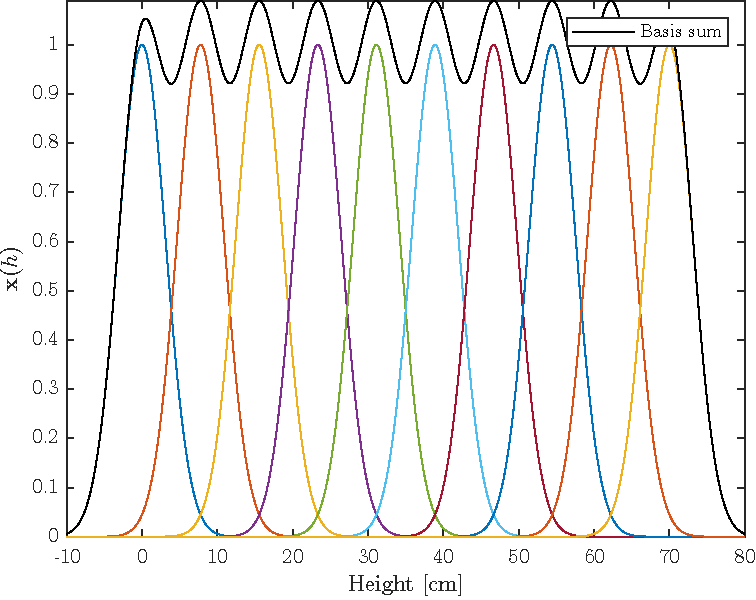
\includegraphics[width=0.7\linewidth]{Figures/RadialSum.pdf}
	\caption{Radial basis functions and their sum.}
	\label{fig:RadialSum}
\end{figure}

The weight vectors update rule will in the continuous height, discrete time and action case be: 

\begin{equation}
	\begin{split}
			\textbf{w}_{t(k),a(k)} \leftarrow \textbf{w}_{t(k),a(k)}
		&+\alpha\bigg[J(k+1)+\gamma\min_{a'}\bigg(\textbf{w}_{t(k+1),a'}^{\intercal}\textbf{x}\bigg(h(k+1)\bigg)\bigg)\\
		&-\textbf{w}_{t(k),a(k)}^{\intercal}\textbf{x}(h\bigg(k)\bigg)
		\bigg]\textbf{x}\bigg(h(k)\bigg)
	\end{split}
\end{equation}

Where $ t(k) $ and $ a(k) $ is taken from finite sets. \cref{alg:FuncApproxQ-learning} presents the function approximation Q-Learning algorithm applied to the water distribution network shown in \cref{sec:WDNsetup}. with continuous height state and discrete time state and discrete actions.

\begin{algorithm}
	\caption{Continuous height discrete time and action Function approximation Q-Learning algorithm}
	\label{alg:FuncApproxQ-learning}
	\begin{algorithmic}[1]
		\State \textbf{Input:} $\alpha\in[0,\;1]$, small $\epsilon>0$, and $0\leq\gamma < 1$, number of Radial basis functions, center placements and width
		
		\State \textbf{Initialise:} weight vectors $ \textbf{w}_{t,a} $ for all discrete times and actions (e.g. $ \textbf{w}_{t,a}=0 $), and states $ t(1) $ and $ h(1) $ 
		
		\For{k=1,2,...}

	\State Take action according to a $\epsilon$-greedy policy:
	\begin{equation*}
		a(k) = \begin{cases} 
			\underset{a'\in \mathcal{A}}{\arg\min} \; \hat{Q}\bigg(h(k),\textbf{w}_{t(k),a'}\bigg) & \text{exploitation with probability} \; 1-\epsilon  \\
			\text{Random action from $ \mathcal{A} $} & \text{exploration with probability} \; \epsilon 
		\end{cases}
	\end{equation*}

\State Observe next states $ h(k+1) $, $ t(k+1) $ and cost $ J(k+1) $

\State Update $ \textbf{w}_{t(k),a(k)} $ according to:
	\begin{equation*}
	\begin{split}
		\textbf{w}_{t(k),a(k)} \leftarrow \textbf{w}_{t(k),a(k)}
		&+\alpha\bigg[J(k+1)+\gamma\min_{a'}\bigg(\textbf{w}_{t(k+1),a'}^{\intercal}\textbf{x}\bigg(h(k+1)\bigg)\bigg)\\
		&-\textbf{w}_{t(k),a(k)}^{\intercal}\textbf{x}\bigg(h(k)\bigg)
		\bigg]\textbf{x}\bigg(h(k)\bigg)
	\end{split}
\end{equation*}
		\EndFor
	\end{algorithmic}
\end{algorithm}

\clearpage \newpage

\subsection{Continuous Height and Time, and Discrete Action}\label{sec:WDN2D}

In the continuous water level and time, and discrete action case, it is necessary to create a weight-vector for every discrete action. 

\begin{equation}\label{eq:Qhat1Discrete}
	\hat{Q}\bigg(h(k),t(k),\textbf{w}_{a}\bigg)=\textbf{w}_{a(k)}^{\intercal}\textbf{x}\bigg(h(k),t(k)\bigg)
\end{equation}

This reduces the number of weight vectors from 96 as in \cref{sec:WDN1D} to only 3. As in \cref{sec:WDN1D} radial basis functions are used as basis function for the height part of the feature vector. Another linear function approximation method is based on Fourier series, which are useful for approximating periodic functions such as water consumption:

\begin{equation}\label{eq:FSApproxDef}
	f(t)=a_{0}+\sum_{n=1}^{n=N}(a_{n}\cos(2\pi n f_{0} t)+b_{n}\sin(2\pi n f_{0}t))
\end{equation}

Where $ a_0, a_{n} $ and $ b_{n} \in \mathbb{R}$ are the Fourier coefficients and $ f_0 $ is the first harmonic of the signal. \cref{eq:FSApproxDef} can be rewritten as a linear combination of weights $ \textbf{w} $ and a feature vector $ \textbf{x} $ containing $\sin$ and $\cos$ basis functions.

\begin{equation}
	f(t)=\textbf{w}^\intercal\textbf{x}(t)
\end{equation}

With weight vector and basis functions defined as:

\begin{equation}\label{eq:wxFS}
	\textbf{w} = 
	\begin{bmatrix}
		a_{0}\\
		a_{1}\\
		b_{1}\\
		a_{2}\\
		\vdots
	\end{bmatrix}
\quad \wedge \quad
	\textbf{x}(t) = 
	\begin{bmatrix}
		1\\
		\sin(2\pi f_0 t)\\
		\cos(2\pi f_0 t)\\
		\sin(4\pi f_0 t)\\
		\vdots \\
	\end{bmatrix} 
\end{equation}

The harmonic frequencies found is based on a fast Fourier transformation of the consumer data described in \cref{sec:Consumption}. From the fast Fourier transform, shown in \cref{fig:FFT}, the demand profile is found to have a major dc-component and frequency-components corresponding to periods of 24 hours, 12 hours, 8 hours, 6 hours, and 4 hours corresponding to the first, second, third, fourth and sixth harmonic. 
 
\clearpage
\begin{figure}[h!]
	\centering
	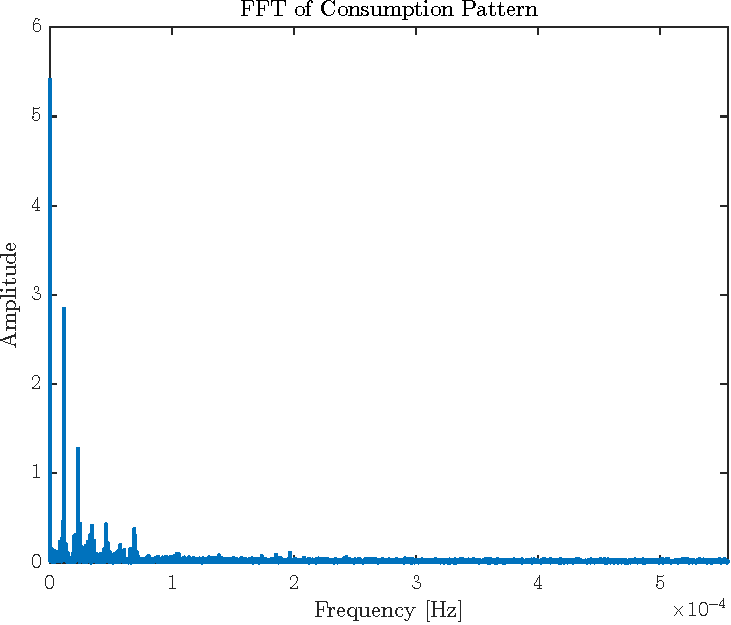
\includegraphics[width=0.7\linewidth]{Figures/FFT.pdf}
	\caption{Fast fourier transformation for consumer data.}
	\label{fig:FFT}
\end{figure} 

The action value function is then approximated as a linear combination of a weight vector and a radial basis function feature vector, and a linear combination of a weight vector containing Fourier coefficients and feature vector according to $ \textbf{x}(t) $ in \cref{eq:wxFS}:

\begin{equation}
	\hat{Q}\bigg(h(k),t(k)\textbf{w}_{a(k)}\bigg)=\textbf{w}_{a(k)}^{\intercal}\textbf{x}\bigg(h(k),t(k)\bigg)=
	\begin{bmatrix}
		\textbf{w}_{a_{RBF}}\\
		\textbf{w}_{a_{FS}}
	\end{bmatrix}^{\intercal}
	\begin{bmatrix}
		\textbf{x}_{RBF}(h)\\
		\textbf{x}_{FS}(t)
	\end{bmatrix}
\end{equation}

The weight vectors update rule is:

\begin{equation}
\begin{split}
	\textbf{w}_{a(k)} \leftarrow \textbf{w}_{a(k)}
	&+\alpha\bigg[J(k+1)+\gamma\min_{a'}\bigg(\textbf{w}_{a'}^{\intercal}\textbf{x}(h(k+1),t(k+1))\bigg)\\
	&-\textbf{w}_{a(k)}^{\intercal}\textbf{x}\bigg(h(k),t(k)\bigg)
	\bigg]\textbf{x}\bigg(h(k),t(k)\bigg)
\end{split}
\end{equation}

\cref{alg:ContFuncApproxQ-learning} presents function approximation Q-Learning algorithm applied to the water distribution network shown in \cref{sec:WDNsetup} with continuous height and time, and discrete actions.

\begin{algorithm}
	\caption{Continuous height and time, discrete action Function Approximation Q-Learning algorithm}
	\label{alg:ContFuncApproxQ-learning}
	\begin{algorithmic}[1]
		\State \textbf{Input:} $\alpha\in[0,\;1]$, small $\epsilon>0$, and $0\leq\gamma < 1$, number of Radial basis functions, center placements, width and number of Fourier Series basis functions
				
		\State \textbf{Initialise:}  weight vectors $ \textbf{w}_{a} $ for all discrete actions (e.g. $ \textbf{w}_{a}=0 $), and states $ t(1) $ and $ h(1) $ 
		
		\For{k=1,2,...}
		
		\State Take action according to a $\epsilon$-greedy policy:
		\begin{equation*}
			a(k) = \begin{cases} 
				\underset{a'\in \mathcal{A}}{\arg\min} \; \hat{Q}\bigg(h(k),t(k),\textbf{w}_{a'}\bigg) & \text{exploitation with probability} \; 1-\epsilon  \\
				\text{Random action from $ \mathcal{A} $} & \text{exploration with probability} \; \epsilon 
			\end{cases}
		\end{equation*}
		
		\State Observe next states $ h(k+1) $, $ t(k+1) $ and cost $ J(k+1) $
		
		\State Update $ \textbf{w}_{a(k)} $ according to:
	\begin{equation*}
		\begin{split}
			\textbf{w}_{a(k)} \leftarrow \textbf{w}_{a(k)}
			&+\alpha\bigg[J(k+1)+\gamma\min_{a'}\bigg(\textbf{w}_{a'}^{\intercal}\textbf{x}(h(k+1),t(k+1))\bigg)\\
			&-\textbf{w}_{a(k)}^{\intercal}\textbf{x}\bigg(h(k),t(k)\bigg)
			\bigg]\textbf{x}\bigg(h(k),t(k)\bigg)
		\end{split}
	\end{equation*}
		\EndFor
	\end{algorithmic}
\end{algorithm}

\clearpage


